\documentclass[11pt]{article}
%\usepackage[T1]{fontenc}
\usepackage{ae,aecompl}
%\usepackage{times} disallowed
%\usepackage{pslatex}
%\usepackage{fullpage}
\usepackage{amssymb,amsmath,amscd,bm}
\usepackage{amsfonts}
\usepackage{url}
\usepackage{boxedminipage}
\usepackage{subfigure}
\usepackage{algorithmic}
\usepackage{algorithm}
\usepackage{amscd}
\usepackage{amstext}
\usepackage{color}
\usepackage{wrapfig}
\usepackage{paralist}
\usepackage{float}
\usepackage{hyperref}
\usepackage{enumitem}
\usepackage{graphicx}
\graphicspath{figures}
\hypersetup{
    colorlinks=true,
    linkcolor=blue,
    filecolor=magenta,      
    urlcolor=cyan,
}
\usepackage{tikz}
\usetikzlibrary{fit,positioning}
\usetikzlibrary{calc}

\setlength{\oddsidemargin}{-0.25in}
\setlength{\evensidemargin}{-0.25in}
\setlength{\topmargin}{-0.25in}
\setlength{\headheight}{0pt}
\setlength{\headsep}{0pt}
\setlength{\footskip}{33pt}
%\setlength{\textheight}{9.25in}
\setlength{\textheight}{9.4in}
\setlength{\textwidth}{7in}
\setlength{\marginparwidth}{0in}
\setlength{\marginparsep}{0in}



%\input{sq}
\def\eqref#1{Eq.~\ref{eq:#1}}
\def\figref#1{Fig.~\ref{fig:#1}}
\def\tabref#1{Tab.~\ref{tab:#1}}
\def\secref#1{Sec.~\ref{sec:#1}}
\def\argmax{\mathop{\rm argmax}}
\def\todo#1{[{\color{red}to-do: \it #1}]}
\def\cjl#1{[{\color{magenta}CJL says: \it #1}]}
\def\csc#1{[{\color{blue}CC says: \it #1}]}
\newcommand{\HRule}{\rule{\linewidth}{0.5mm}}

\usepackage[skins,breakable]{tcolorbox}

\newtcolorbox[]{solution}[1][]{
% answer formatting
title=Solution,
breakable
}

\long\def\gobble#1{}
\long\def\squelch#1#2{#2}
\def\argmin{\mathop{\rm argmin}}
\def\argmax{\mathop{\rm argmax}}



\newenvironment{closeitemize}{\begin{itemize}\topsep=0in\itemsep=0in\parsep=0in}{\end{itemize}}
\newenvironment{closeenum}{\begin{enumerate}\topsep=0in\itemsep=0in\parsep=0in}{\end{enumerate}}
\newcommand{\tikzmark}[1]{%
  \tikz[overlay,remember picture] \node (#1) {};}

\def\ourtitle{MSCBIO 2070/02-710: Computational Genomics, Spring 2022\\ \\
HW3: Genomics in the Real World \\ \\
{\small\em Version: 1\\Due: 11:59 EST, March 30, 2022 by Gradescope\\
}
}

\begin{document}

\thispagestyle{empty}
\setcounter{page}{1}

\noindent {\large\bf \ourtitle} \vspace*{0.5em} \\
\vspace{0.05in}
\HRule
\vspace*{0.1in}    

\noindent 
{\bf Topics} in this assignment: 
\begin{enumerate}
\item ChIP seq analysis
\item Linkage disequilibrium
\item Hardy-Weinberg equilibrium
\end{enumerate}
\vspace{0.2in}


All data for this assignment is available for download \href{https://cmu.box.com/s/3svqmspc8xou4peq00qpab6zlh9elrtj}{here}.
\vspace{0.2in}

\noindent 
{\bf What to hand in}. 
\begin{itemize}
\item One write-up (\underline{\textbf{in pdf format}}) addressing each of following questions (this will be an assignment on Gradescope).
\item All source code (this will be a separate assignment on Gradescope). Parts of your code will be autograded, and other parts may be graded by hand. Please make clear in your code (i.e. with comments) which parts you used for which plots/analysis.
\end{itemize}

\textbf{It is highly recommended that you typeset your write-up. Illegible handwriting will not be graded.}\\



\newpage
\begin{enumerate}
\item {\bf [24 points] ChIP-seq analysis.}
\vspace{2mm}

We provide you some ChIP-seq peak data in \texttt{peak.bed} that contains the chromosome, start and end positions of the ChiP-seq peaks from an experiment. This is real transcription factor ChIP-Seq data from a cancer cell line, and your goal is to figure out if you can distinguish what transcription factor the experiment was performed with. In doing so, you will gain familiarity with some common genomics tools.
Most of the parts in this question are pretty open-ended; as long as your answers are well-supported, you will get credit.

\textbf{Data Processing Steps}

Using \texttt{peak.bed}, please complete the following tasks.
\begin{itemize}
\item Using your tool of choice, extract the first 100 lines of this file to a new file \texttt{"trimmed.bed"}.
\item 

        Load \texttt{"trimmed.bed"} in the UCSC Genome Browser (\url{https://genome.ucsc.edu}) as a custom track (use hg19 as the assembly). Get the genomic sequence for each of the intervals through UCSC Genome Browser. You can do that by going to Table Browser in UCSC Genome Browser, select custom track and load \texttt{"trimmed.bed"}, select output format as \textbf{sequence} and get output. Figure \ref{fig:genomebrowser} shows how to do this.

\begin{figure}[h]
\centering
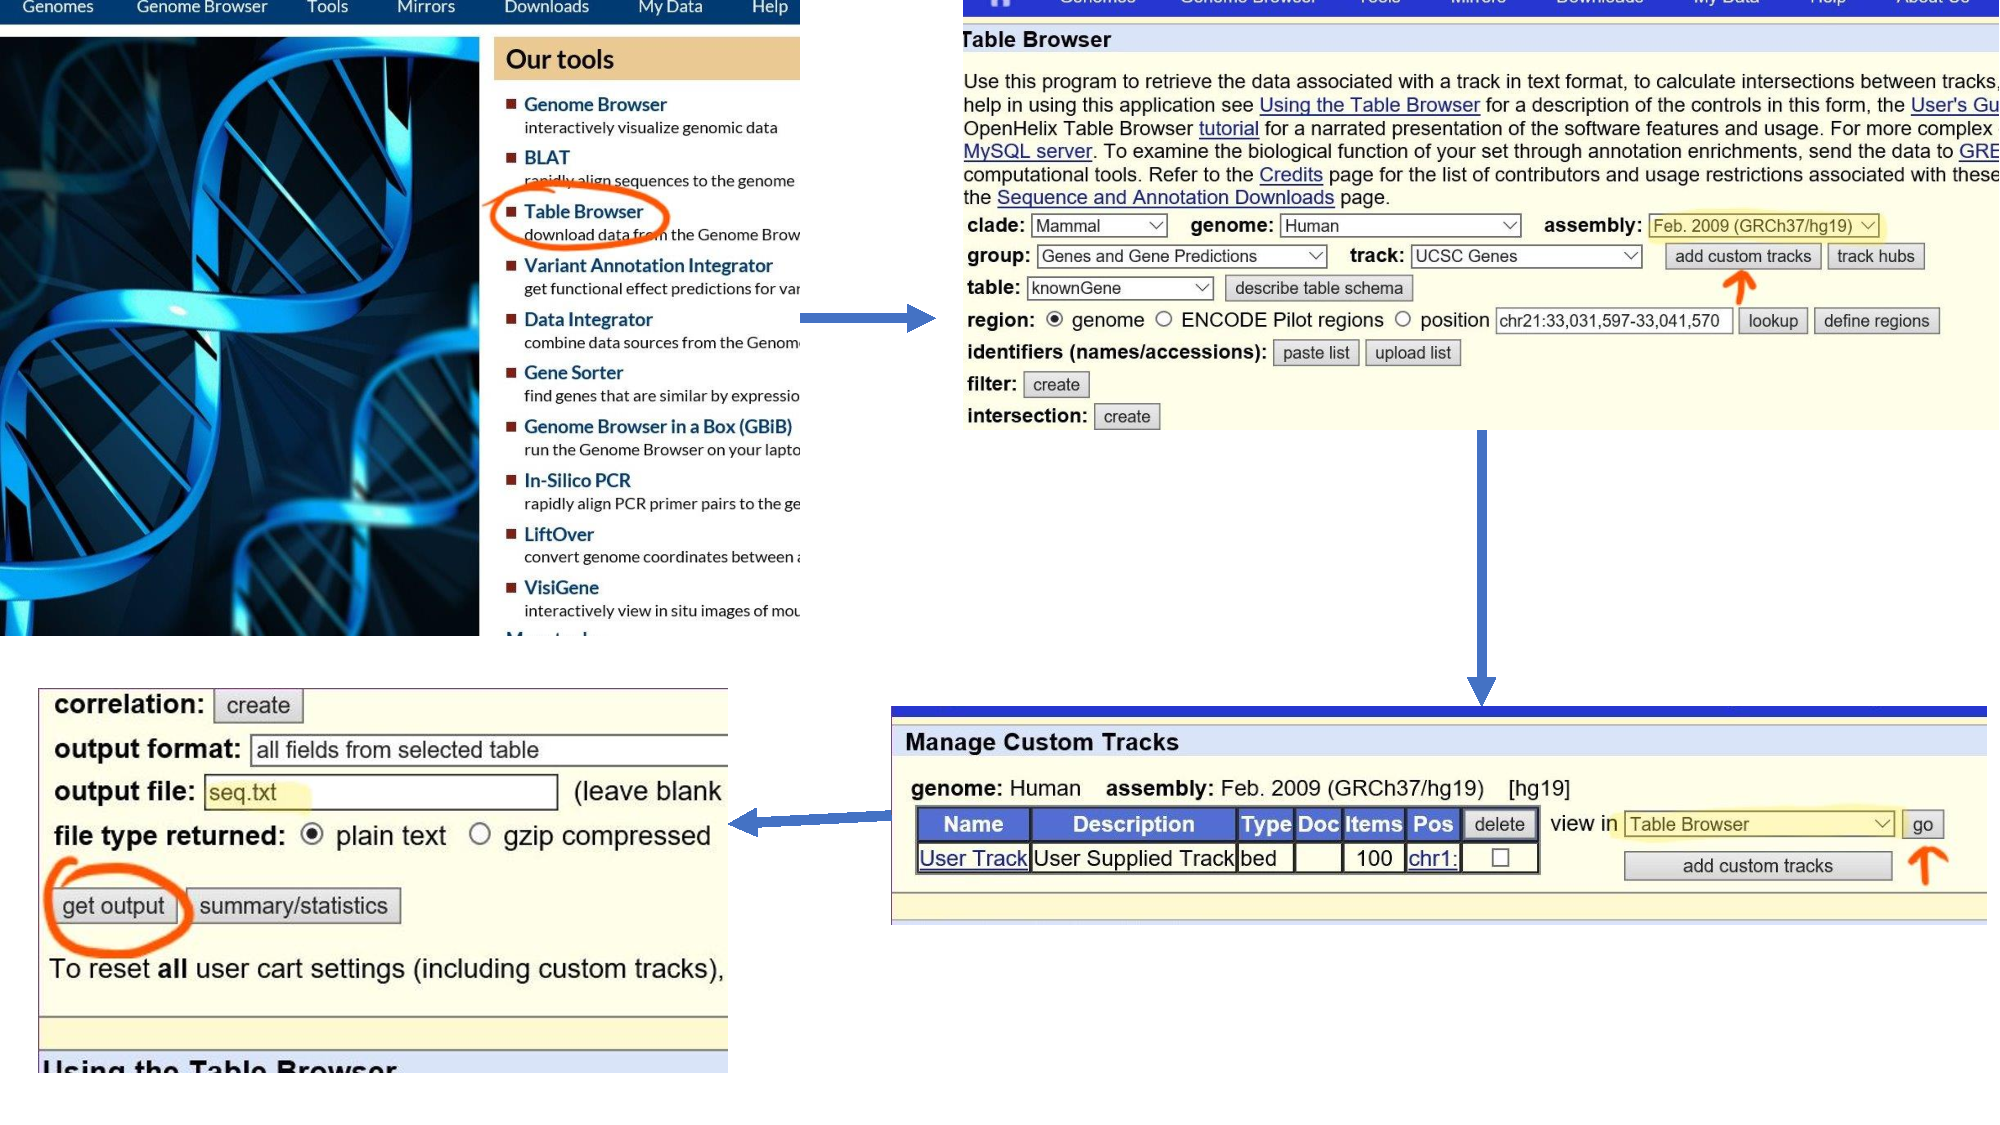
\includegraphics[width=0.8\textwidth]{tuts}
\caption{Use UCSC Table Browser to get the sequence.}
\label{fig:genomebrowser}
\end{figure}
    \item Use MEME (\url{http://meme-suite.org/tools/meme}) to call enriched motifs based on the output sequence. Use the default setting in MEME but only consider output motif with width from 5 to 9 (set under ``Advanced options''). Note that you may still need to adjust the size of the input file to keep the number of characters within 60,000 in the file. You may want to provide your email if you want a notification for when your results are ready from MEME. This may take some time, depending on the server load.
    \item Using each of your hits from MEME, feed them to TOMTOM by clicking the 'submit/download' arrow to the right of your MEME results. Use all default options for TOMTOM.
\end{itemize}



\textbf{Questions}
\begin{enumerate}

\item (2 points) Question -- Screenshot the output returned by MEME.  Based on the motif logos, which one is the most promising hit?


%%%%%%%%%%%%%%%%%%
\begin{solution}
\end{solution}
%%%%%%%%%%%%%%%%%%


\item (6 points) Question -- What is the top hit obtained from TomTom for each of the motifs from MEME? Based on this do you agree with your previous assessment? Note that the E-value reported by TOMTOM is the Bonferroni-corrected p-value.


%%%%%%%%%%%%%%%%%%
\begin{solution}
\end{solution}
%%%%%%%%%%%%%%%%%%


\item (8 points) Question -- Use the original peak.bed file and use GREAT (\url{http://great.stanford.edu/public/html/}) with default settings to identify enriched biological processes and pathways. \textbf{Be sure to use GREAT version 3.0.0, with species hg19.} Screenshot the top five Go Biological Process hits. How do these pathways compare to your expectations based on your MEME results? Would you consider these pathways statistically significant? Hint: explain what the important enrichment statistics mean.
 
 
%%%%%%%%%%%%%%%%%%
\begin{solution}
\end{solution}
%%%%%%%%%%%%%%%%%%


\item (2 points) Question -- Now take a quick look at the hits in the category MSigDB Preturbation category. Explain what type of data is shown here. How much might these hits depend on what type of cancer cells the experiment was done with?

%%%%%%%%%%%%%%%%%%
\begin{solution}
\end{solution}
%%%%%%%%%%%%%%%%%%

\item (6 points) Question -- Suppose that you were interested in determining what type of cancer the provided data was collected from.  Based on your GREAT analyses, how useful is the provided TF ChIP-Seq data for this purpose? Justify this with some explanation: this will require that you understand what the GO terms are, and what processes your TF(s) are involved with. Then outline a follow up high throughput sequencing experiment from those mentioned in class that might help you with this new objective. 

%%%%%%%%%%%%%%%%%%
\begin{solution}
\end{solution}
%%%%%%%%%%%%%%%%%%

\end{enumerate}
 \clearpage
\item {\bf [50 points] Linkage Disequilibrium}

\vspace{2mm}
In this problem we will use genotype sequences for the first $5,000$ SNPS in mouse chromosome 1, derived from a case study involving $1,063$ mice; these data are contained in the file \texttt{chromosome\_1\_phased\_first\_5000\_snps.vcf} (you can read more about this file format \href{http://faculty.washington.edu/browning/beagle/intro-to-vcf.html}{here}). Usually, after sequencing each sample's genome, you would have to phase the sequences (assign each of two alleles at an SNP site to the maternal or paternal chromosome) using a tool like Beagle. However, we have already done this for you, so you are provided as input the phased haplotype data. \\

\fbox{\parbox{0.9\textwidth}{
\textbf{Note: }{Your code is graded by an autograder. You have been given a code skeleton in \texttt{linkage\_disequilibrium.py}. You must complete 6 functions (\texttt{split\_phased\_snps},\\ \texttt{compute\_allele\_frequencies}, \texttt{compute\_haplotype\_frequencies}, \texttt{estimate\_D}, \\ \texttt{estimate\_D\_prime} and \texttt{compute\_r\_squared}).  At the end, the script should be able to run with the following command:\\

\texttt{python linkage\_disequilibrium.py} \\

The formats of arguments and return values of each function are explicitly described in the skeleton code. For the hyperparameters, please use the \textbf{default} values specified in the skeleton code. 
}
}
}

\vspace{2mm}

\begin{enumerate}
    \item (15 points) Complete the \texttt{split\_phased\_snps},
    \texttt{compute\_allele\_frequencies} and \\
    \texttt{compute\_haplotype\_frequencies} functions. \\
    
    The \texttt{split\_phased\_snps} function takes as input a Pandas DataFrame of dimensions \texttt{num\_snps $\times$ num\_samples} which contains phased haplotype data - that is, each element in the array is a string of the form 
    $$\texttt{"maternal\_chromosome\_allele | paternal\_chromosome\_allele"}$$
    
    Here, a \texttt{0} indicates that the allele is the reference allele, whereas a \texttt{1} indicates that the allele is the alternate allele. For example, if an entry in the dataframe is \texttt{0 | 1}, the reference allele at that position is \texttt{G} and the alternate allele at that position is \texttt{A}, then according to the entry the maternal chromosome allele is \texttt{G} and the paternal chromosome allele is \texttt{A}. The output of this function should be a Numpy array of dimensions \texttt{2 $\times$ num\_snps $\times$ num\_samples}, where the last dimension holds the data for the maternal and paternal chromosome separately.\\
    
    The \texttt{compute\_allele\_frequencies} function should calculate the frequency of the reference and alternate alleles for each SNP, so the output should be a $2$-tuple of Numpy arrays, each with length \texttt{num\_snps}. \\
    
    The \texttt{compute\_haplotype\_frequencies} function should calculate the frequency of each of four haplotypes (\texttt{(1, 1)}, \texttt{(1, 0)}, \texttt{(0, 1)}, and \texttt{(0, 0)}) for each pair of SNPs; thus, the output should be a $4$-tuple of Numpy arrays, each with dimensions \texttt{num\_snps $\times$ num\_snps}.

\end{enumerate}        
    Next, we would like to compute the linkage disequilibrium between every pair of SNPs. Suppose that we have two SNPs, one at locus $p$ and the other at locus $q$. Define two indicator variables $P \sim \text{Bernoulli}(p_1)$ and $Q\sim \text{Bernoulli}(q_1)$ which take the value of $1$ when the respective SNP contains the reference allele and a value of $0$ when it contains the alternate allele. Furthermore, let's denote \begin{align*}
        p_0 &= 1 - p_1 \\
        q_0 &= 1 - q_1 \\
        p_{11} &= \mathbb{P}(P = 1, Q = 1) \\
        p_{10} &= \mathbb{P}(P = 1, Q = 0) \\
        p_{01} &= \mathbb{P}(P = 0, Q = 1) \\
        p_{00} &= \mathbb{P}(P = 0, Q = 0)
    \end{align*}

    Essentially, the $p_{ij}$ indicate the probability that $P = i$ \textbf{and} that $Q=j$. In practice,  can estimate these probabilities empirically from our data. \\
    
    Note that, assuming the SNPs are independently inherited, we should have that $p_{ij} = p_{i} \cdot p_{j}$. Thus, we can define the \textit{linkage disequilibrium} ($D$) as the difference between these two quantities. For clarity, here is a table showing the relationships between these quantities:
    \begin{center}
        \begin{tabular}{|c|c|c|}
        \hline
             & Q=1& Q=0\\
        \hline
             P=1& $p_{1}q_{1} + D = p_{11}$& $p_{1}q_{0} - D = p_{10}$\\
        \hline
             P=0& $p_{0}q_{1} - D = p_{01}$& $p_{0}q_{0} + D = p_{00}$ \\
        \hline
        \end{tabular}        
    \end{center}

\begin{enumerate}[resume]
    \item (5 points) Naively, we could estimate $D = p_{11} - p_{1}q_{1}$; however, this would not make full use of all the haplotype frequencies that we have estimated. Show that $$D=p_{11} \cdot p_{00} - p_{10} \cdot p_{01}$$
    is also a valid estimator for $D$.
%%%%%%%%%%%%%%%%%%
    \begin{solution}
    \end{solution}
%%%%%%%%%%%%%%%%%%
\end{enumerate}
Next, we can implement the computation of $D$ to compare the linkage disequilibrium of different SNPs. However, notice that $D$ can take on negative values even though frequencies cannot be negative; this makes it difficult to compare $D$ values. To address this, we can divide $D$ by $D_{max}$, defined as follows:
    \begin{align*}
        D &= p_{11} \cdot p_{00} - p_{10} \cdot p_{01} \\
        D' &= | D / D_{\text{max}} | \text{, where} \\
        D_{\text{max}} &= \begin{cases}
        \min(p_1q_2, p_2q_1), & D > 0 \\
        \max(-p_1q_1, -p_2q_2), & D <= 0 \\
        \end{cases}
    \end{align*}
    This adjustment guarantees that $D'$ lies in the range $[0, 1]$.
    
\begin{enumerate}[resume]
    \item (10 points) Implement \texttt{calculate\_D} and \texttt{calculate\_D\_prime} as described above. Attach a heatmap displaying the square matrix of $D'$ values, with brighter colors indicating a value near $1$ and darker colors indicating values near $0$. From the plot, you should be able to identify linkage blocks - that is, adjacent regions of the DNA that are inherited together and show complete linkage disequilibrium (there should be anywhere from $5 - 10$ of these of varying sizes, depending on how stringent of a criterion you use for defining them). How big is the biggest clear linkage block, in terms of the number of SNPs spanned (a rough estimate is enough)? How small is the smallest clear linkage block? \\
    
    \textbf{Hint \#1:} Note that the $D'$ matrix is symemtric, so you only need to calculate its values for either the upper or lower triangular values of the matrix.
    
    \textbf{Hint \#2:} Make sure to vectorize your calculations as much as possible to ensure a reasonable runtime. With an efficient implementation, your code should for this part shouldn't run for longer than $10$ minutes. For debugging, you can try testing on just a subset of the SNPs.

%%%%%%%%%%%%%%%%%%    
    \begin{solution}
    \end{solution}
%%%%%%%%%%%%%%%%%%
\end{enumerate}

Another common measure of the linkage disequilibrium between two loci is $r^2$, the square of Pearson's correlation coefficient. Pearson's correlation coefficient for two variables $X$ and $Y$ is defined as follows:
\begin{align*}
    r(X, Y) &= \frac{\text{cov}(X, Y)}{\sigma_{X}\sigma_{Y}}\text{, where} \\
    \text{cov}(X, Y) &= \mathbb{E}[(X - \mathbb{E}[X])(Y - \mathbb{E}[Y])] \\
    \sigma^2_{X} &= \mathbb{E}[(X - \mathbb{E}[X])^2] 
\end{align*}
In other words, $\text{cov}(X, Y)$ is the covariance of $X$ and $Y$ and $\sigma^2_{X}$ is the variance of $X$.\\

\begin{enumerate}[resume]
    \item (10 points) 
    Show that, for indicator variables $P \sim \text{Bernoulli}(p_1)$ and $Q \sim \text{Bernoulli}(q_1)$, $$r(P, Q) \approx \frac{D}{\sqrt{p_1p_2q_1q_2}}$$
    where $D = p_{11} - p_1q_1$ is the linkage disequilibrium as calculated in part (b). Note that we use the naive definition of $D$ for this proof. \\
    
    \textbf{Hint:} Recall that the variance of a Bernoulli variable $X$ with parameter $p$ is $\sigma^2_X = p(1-p)$.

%%%%%%%%%%%%%%%%%%
    \begin{solution}
    \end{solution}
%%%%%%%%%%%%%%%%%%

    \item (10 points) Using the formula that you derived in part (c), implement \texttt{calculate\_r\_squared}. Attach a heatmap of the square matrix of $r^2$ values, similar to part (d). Compare to the heatmap in (d); qualitatively, what similarities/differences do you notice? 
%%%%%%%%%%%%%%%%%%
    \begin{solution}
    \end{solution}
%%%%%%%%%%%%%%%%%%
\end{enumerate}
\newpage
 \clearpage
\item {\bf [26 points] Hardy-Weinberg Equilibrium}

\vspace{2mm}
In this problem, we will leverage the phasing of the haplotype data in order to derive aspects about the structure of the population that we are working with;. Here we will use all the SNPs from chromosome $19$ for the same $1,063$ mice that we used in the previous problem; these data are contained in the file \texttt{chromosome\_19\_phased\_snps.vcf}

\fbox{\parbox{0.9\textwidth}{
\textbf{Note: }{Your code is graded by an autograder. You have been given a code skeleton in \texttt{population\_structure.py}. You must complete 4 functions \texttt{compute\_effective\_allele\_frequencies},\\ \texttt{compute\_genotype\_counts}, \texttt{calculate\_chi\_squared\_statistic}, \\ \texttt{detect\_snps\_under\_selection}).  At the end, the script should be able to run with the following command:\\

\texttt{python hardy\_weinberg.py} \\

The formats of arguments and return values of each function are explicitly described in the skeleton code. For the hyperparameters, please use the \textbf{default} values specified in the skeleton code. 
}
}
}

First, we will use the Hardy-Weinberg test. 
The Hardy-Weinberg test evaluates whether or not a genomic locus violates the Hardy-Weinberg equilibrium. The statistic can be written as follows
$$\chi^2 = \sum_{i= 1}^{\text{\# of categories}} \frac{(\text{observed count}_i - \text{expected count}_i)^2}{\text{expected count}_i}$$
For our application, we have three categories at each locus (homozygous dominant, heterozygous and homozygous recessive). After computing the $\chi^2$ statistic, we can compare it to a threshold based on our significance level and the degrees-of-freedom parameter to detect SNPs under selection.
\begin{enumerate}
    \item (10 points) Implement the  \texttt{compute\_effective\_allele\_frequencies} and \texttt{compute\_genotype\_counts} functions. These will be used for computing the $\chi^2$ statistic in part (b).
    
    \textbf{Note:} For this problem, you will calculate the effective allele frequencies in a slightly different way from how you calculated them in the previous problem. In particular, if you have that $c_{11}$ is the number of $\texttt{"0" | "0"}$ genotypes observed, $c_{12}$ is the number of $\texttt{"0" | "1"}$ genotypes observed, $c_{21}$ is the number of $\texttt{"1" | "0"}$ genotypes observed and $c_{00}$ is the number of $\texttt{"1" | "1"}$, then the frequency of the reference allele is $\frac{2c_{11} + (c_{21} + c_{12})}{2(c_{11} + c_{21} + c_{12} + c_{22})}$; the complement holds for the frequency of the alternate.
    
    \item (11 points) Implement the \texttt{calculate\_chi\_squared\_statistic} and \texttt{detect\_snps\_under\_selection} functions. Use these functions to identify SNPs that are actively under selection. Using a significance level $=0.01$ and degrees-of-freedom $=1$, what fraction of SNPs from the sample violate Hardy-Weinberg equilibrium?\\
    
    \textbf{Hint:} Use \href{https://docs.scipy.org/doc/scipy/reference/generated/scipy.stats.chi2.html}{\texttt{scipy.stats.distributions.chi2}}'s \texttt{ppf} method to calculate the correct threshold for significance.
%%%%%%%%%%%%%%%%%%
    \begin{solution}
    \end{solution}
%%%%%%%%%%%%%%%%%%
    \item (5 points) For a $\chi^2$ test, we must first specify the degrees-of-freedom parameter. This parameter is the number of freely varying factors in our data, and it governs the shape of the $\chi^2$ distribution. In applications to genotypic frequencies, despite the fact that there are three different categories, we usually use a value of $1$ for the degrees-of-freedom parameter. Why is this?
    
    \begin{solution}
    
    \end{solution}
\end{enumerate}
\newpage
 \clearpage
\end{enumerate}

\end{document}
